\section{Modelli per sistemi paralleli}
E' qualcosa di complesso che richiede una parte HW e software, bisogna necessariamente fare delle astrazioni perche' non ci potremo occupare di tutti i dettagli.
Abbiamo questa astrazione:
\begin{itemize}
    \item Livello macchina: assembly
    \item Modello architetturale: SIMD o MIMD, si prevedono anche processi in cui ci sono tante unita' di calcolo che interagiscono tra di loro, gestione multi processi e multi thread
    \item Modello computazionale: e' un modello formale che consente di descrivere la macchina astraendo dai modello sottostanti ed e' fondamentale per la creazione degli algoritmi. Processore, memoria, scambio dati con un BUS. E' inerentemente sequenziale ma e' utile per creare l'algoritmo data la size dei dati. Nell'ambito del parallelismo passiamo dal modello RAM al PRAM (modello RAM per architetture parallele)
    \item Modello di programmazione parallela: e' il modo con cui gestiamo il sistema di calcolo parallelo esprimendo algoritmi con un linguaggio che espone il prallelismo dell'architettura sottostante per essere eseuito da un linguaggio che ha in se elementi che permettono di usare il parallalismo. Vi sono aspetti di comunicazione per gestire il multi threading, si affronta quindi la suddivisione del compito in processi e thread. Fino ad arrivare a problemi legati all'uso o della gestione di spazi di indirizzamento condivisi.
\end{itemize}

\subsection{SIMD}
Si parla di unita' molteplici che lavorano sui dati, laddove i dati permettono di sviluppare meccanismi paralleli. E' un mondo vasto che si puo' vedere anche nelle architetture comuni dove si ha la divisione di computazione in diverse ALU specializzate, una che lavora su un singolo registro ed una che lavora vettorialmente ed e' quindi in grado di lavorare su piu' dati contemporaneamente. Nelle GPU parleremo di thread che lavorano simultaneamente in modalita' SIMD.

\subsection{MIMD}
E' un'altro dei modelli molto diffusi paralleli in cui si hanno le istruzioni di tanti dati simultaneamente che vengono eseguite da un numero di processori veramente grandi.

\subsection{PRAM}
Il modello PRAM e' il modello di calcolo parallelo piu' semplice, in questo caso abbiamo una memoria condivisa, i processori lavorano in maniera SIMD ovvero fanno la stessa istruzione, esistono anche processori inattivi.
Ci da quanti passi ci servono per risolvere l'algoritmo parallelo, anche in questo caso potremmo fare studio di complessita' per risolvere il problema parallelo.

\subsection{Parallelizzazione di algoritmi}
Quando vorremo vedere la complessita' computazionale degli algoritmi dovremo fare delle astrazioni ed usare qualcosa simile al PRAM.
Nella pratica si partira' da un algoritmo sequenziale, dovremo vedere come dividere la computazione in parallelo per capire come le varie parti vengano attribuite ai vari thread, tendenzialmente la partizione logica dei task la faremo noi, la parte dello scheduling se ne occupa il sistema ma e' bene conoscela perche' ad esempio in CUDA i processi di scheduling sono fortemente condizionanti dalla potenza del sistema e dovremo adeguare gli algoritmi sulla base dei meccanismi di scheduling. Quello che vorremo ottenere e' una massima occupancy delle unita' di calcolo.
Dipendentemente dal modello di memoria, un task può accedere a memoria condivisa o usare tecniche di message passing.

\section{CPU multi-core e programmazione multi-threading}
Un programma in esecuzione e' un processo che viene allocato nel OS e ha una serie di risorse che ha, convive con altri processi nel sistema ed e' una cosa abbastanza pesante, mentre i thread che compongono un processo sono dei sotto-processi ma piu' leggeri. Un processo in genere consiste di tanti thread. In genere vengono creati da delle operazioni di sistema come le fork in UNIX e vengono terminati dall'OS.
I processi hanno il loro contesto e vengono eseguit sequenzialmente secondo un flusso, anche i thread eseguono le cose sequenzialmente ma essendo molteplici possono essere parallali.
Il thread e' un singolo flusso di istruzione che si trova in un processo che lo scheduler si occupa di eseguire concorrentemente ad altri threads.

\subsection{Thread}
Ha un ciclo di vita, viene generato e viene ucciso, il processo chiude quando tutti i thread hanno terminato la loro esecuzione:
\begin{itemize}
    \item New: viene generato, chi lo ha generato sa chi e' 
    \item Executable: il thread e' pronto per essere eseguito quando ha tutte le risorse necessarie
    \item Running: il thread sta attualmente eseguendo le sue istruzioni
    \item Waiting: il thread sta aspettando che una risorsa diventi disponibile
    \item Finished: il thread ha completato la sua esecuzione e viene rimosso
\end{itemize}

\begin{figure}[ht!]
    \centering
    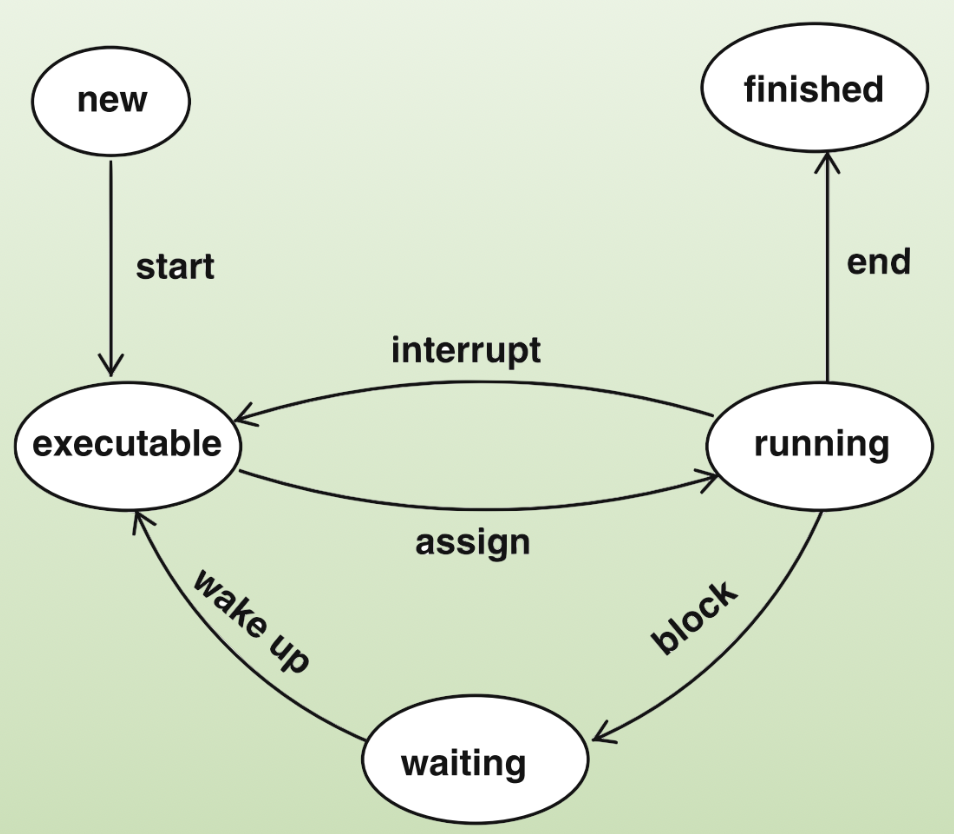
\includegraphics[width=0.5\textwidth]{images/statiThread.png}
    \caption{Stati di un thread}
\end{figure}

I vantaggi sono:
\begin{itemize}
    \item Si possono avere tanti flussi di esecuzioni che possono avvantaggiarsi di sistemi multi-core
    \item Visibilita' dei dati globale
    \item Semplicita' di gestione eventi asincroni come l'io 
    \item Velocita' di context switching
\end{itemize}

Le difficolta' sono la concorrenza e il problema di avere uno spazio privato.

\section{Programmazione multi-core}
Noi vedremo la programmazione multi-thread su architetture multi-core. L'applicazione deve essere progettata considerando diversi fattori del sistema di calcolo parallelo multi-core (e many core come le GPU), bisogna trovare di task, bilanciarli, suddividere i dati sui vari task (il problema e i dati lo devono consentire) e farlo in modo che tutti i task possano lavorare su queste porzioni di dati indipendentemente. Ci sono quindi tanti aspetti da tenere in considerazione sulla dipendenza e indipendenza dei dati. Test e debugging sono anchessi importanti quando si sviluppano gli algoritmi in ambito parallelo perche' ci sono tanti flussi di esecuzione.

\section{Programmazione CUDA}
Pensare in parallelo significa avere chiaro quali feature la GPU espone al programmatore. Si lavora come su pthread o OpenMP. Si scrive una porzione di CUDA C (semplice estensione di C) per l'esecuzione sequenziale e lo si estende a migliaia di thread (permette di pensare 'ancora' in sequenziale)

\begin{itemize}
    \item I dati stanno su host
    \item allocare spazio su GPU
    \item copiare i dati da host a GPU
    \item allocare memoria per l'output
    \item lanciare il kernel che elabora dati in ingresso e li mette in output, mette una copia su memoria condivisa
    \item cancellare le memorie allocate
\end{itemize}

\subsection{Organizzazione dei thread}
Cuda presenta una gerarchia astratta di thread che si distribuisce su due livelli:
\begin{itemize}
    \item grid: una griglia ordinata di blocchi
    \item block: un insieme di thread che possono cooperare tra loro
\end{itemize}
Questi possono avere dimensioni 1D, 2D o 3D. Tutto questo fa 9 combinazioni tra grid e block.

\begin{figure}[ht!]
    \centering
    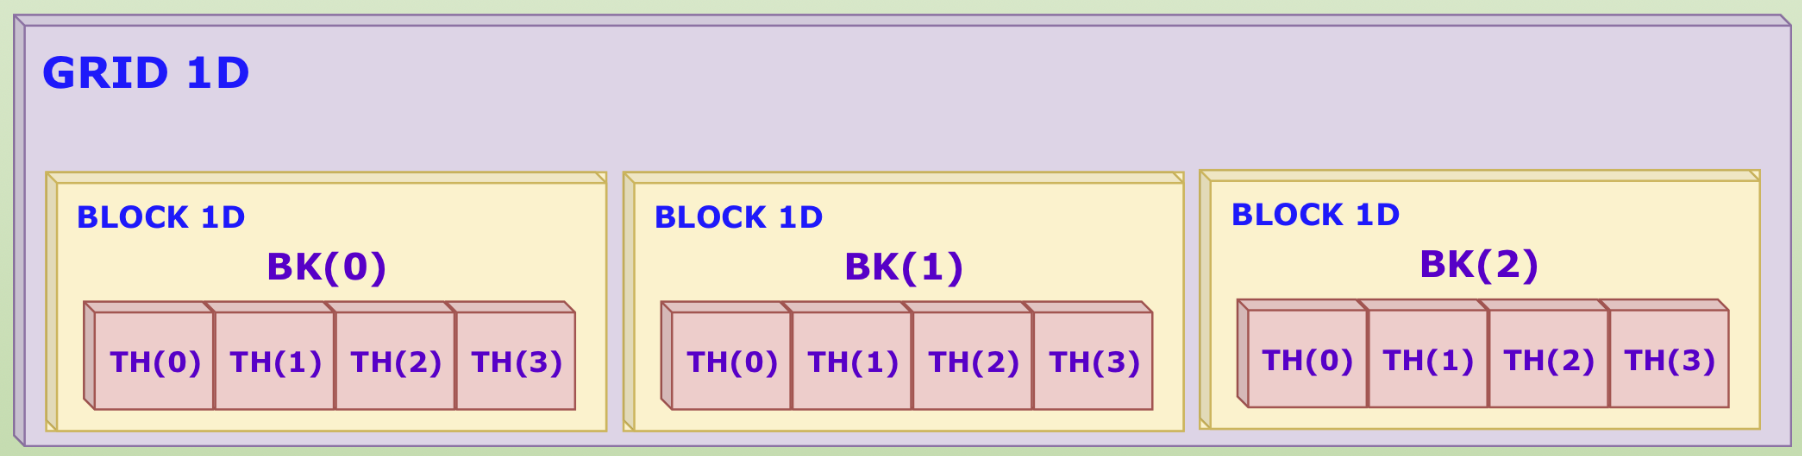
\includegraphics[width=0.5\textwidth]{images/organizzazioneThread.png}
    \caption{Organizzazione dei thread in CUDA}
\end{figure}

Ci sono delle limitazioni, un blocco puo' contenere al massimo 1024 thread.

Il blocco di thread e' molto importante, dal punto di vista semantico ha un significato, e' un gruppo di thread che possono cooperare tra loro tramite:
\begin{itemize}
    \item block-local synchronization, sincronizzazione: cooperare per uno stesso compito avvantaggiandosi da operazioni fatte da altri thread
    \item block-local communication, comunicazione tramite la shared memory: e' una memoria cache che quindi ha tempi di accesso di molto ridotti
\end{itemize}

I thread vengono identificati univocamente tramite l'id di blocco e l'id di thread. blockIdx e threadIdx sono specificati in variabili globali, un kernel a runtime ha accesso a queste informazioni che vengono assegnate dinamicamente, hanno tre valori x, y, z di tipo uint32.

\begin{lstlisting}[language=C]
    
#include <stdio.h>

__global__ void checkIndex(void) {
	printf("threadIdx:(%d, %d, %d) blockIdx:(%d, %d, %d) "
					"blockDim:(%d, %d, %d) gridDim:(%d, %d, %d)\n",
					threadIdx.x, threadIdx.y, threadIdx.z,
					blockIdx.x, blockIdx.y, blockIdx.z,
					blockDim.x, blockDim.y, blockDim.z,
					gridDim.x,gridDim.y,gridDim.z);
}

/*
* MAIN
*/
int main(int argc, char **argv) {

	// grid and block definition
	dim3 block(4);
	dim3 grid(3);

	// Print from host
	printf("Print from host:\n");
	printf("grid.x = %d\t grid.y = %d\t grid.z = %d\n", grid.x, grid.y, grid.z);
	printf("block.x = %d\t block.y = %d\t block.z %d\n\n", block.x, block.y, block.z);

	// Print from device
	printf("Print from device:\n");
	checkIndex<<<grid, block>>>();

	// reset device
	cudaDeviceReset();
	return(0);
}
\end{lstlisting}
Abbiamo accesso alle dimensioni della griglia e del blocco tramite le variabili blockDim e gridDim, che sono anchessi di tipo uint32. Anche in questo caso abbiamo tre componenti x, y, z.

L'indice univoco del thread nei blocchi si calcola differentemente rispetto alle dimensioni del blocco:

\begin{figure}[ht!]
    \centering
    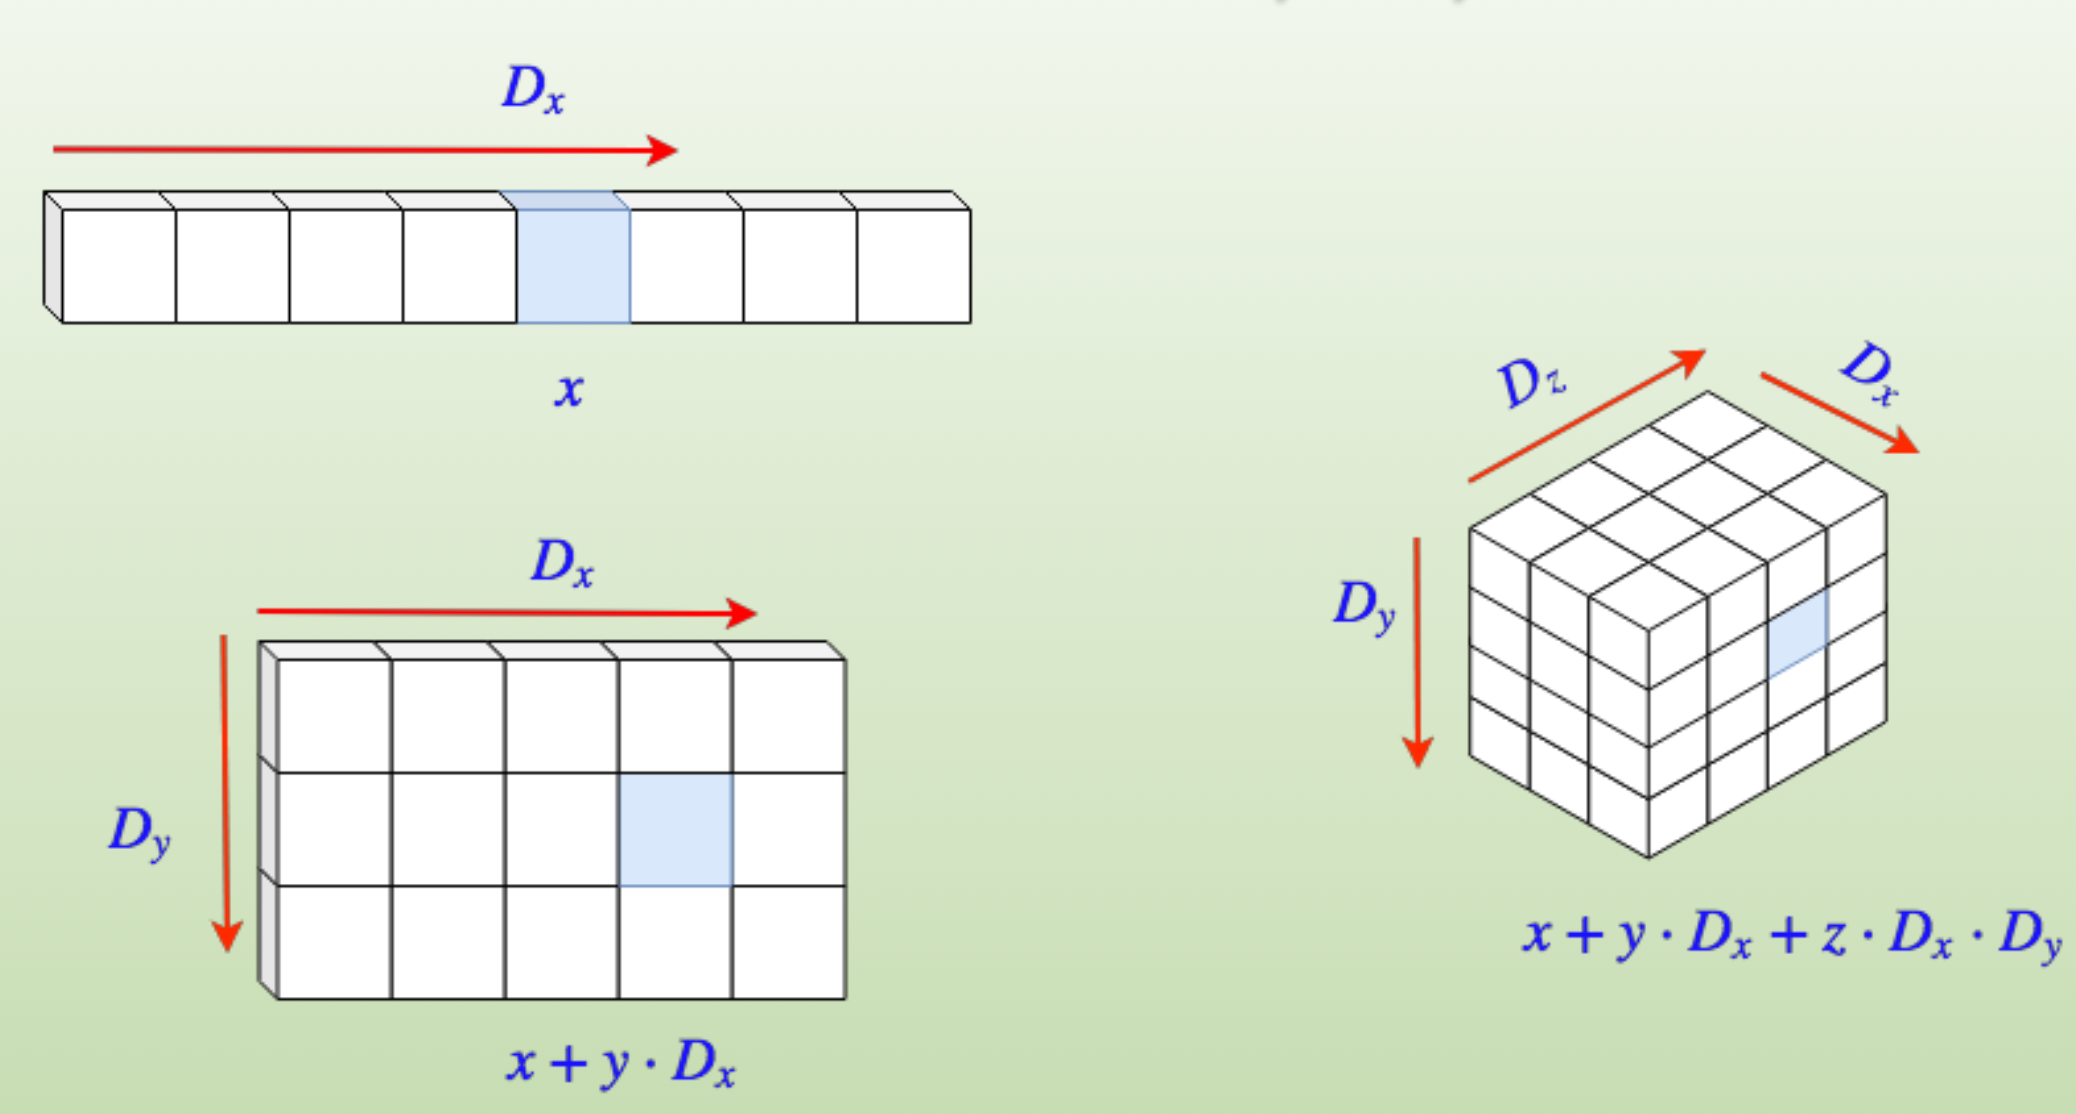
\includegraphics[width=0.8\textwidth]{images/indiceUnicoBlocchi.png}
    \caption{Indice univoco dei thread nei blocchi}
\end{figure}


\begin{figure}[ht!]
    \centering
    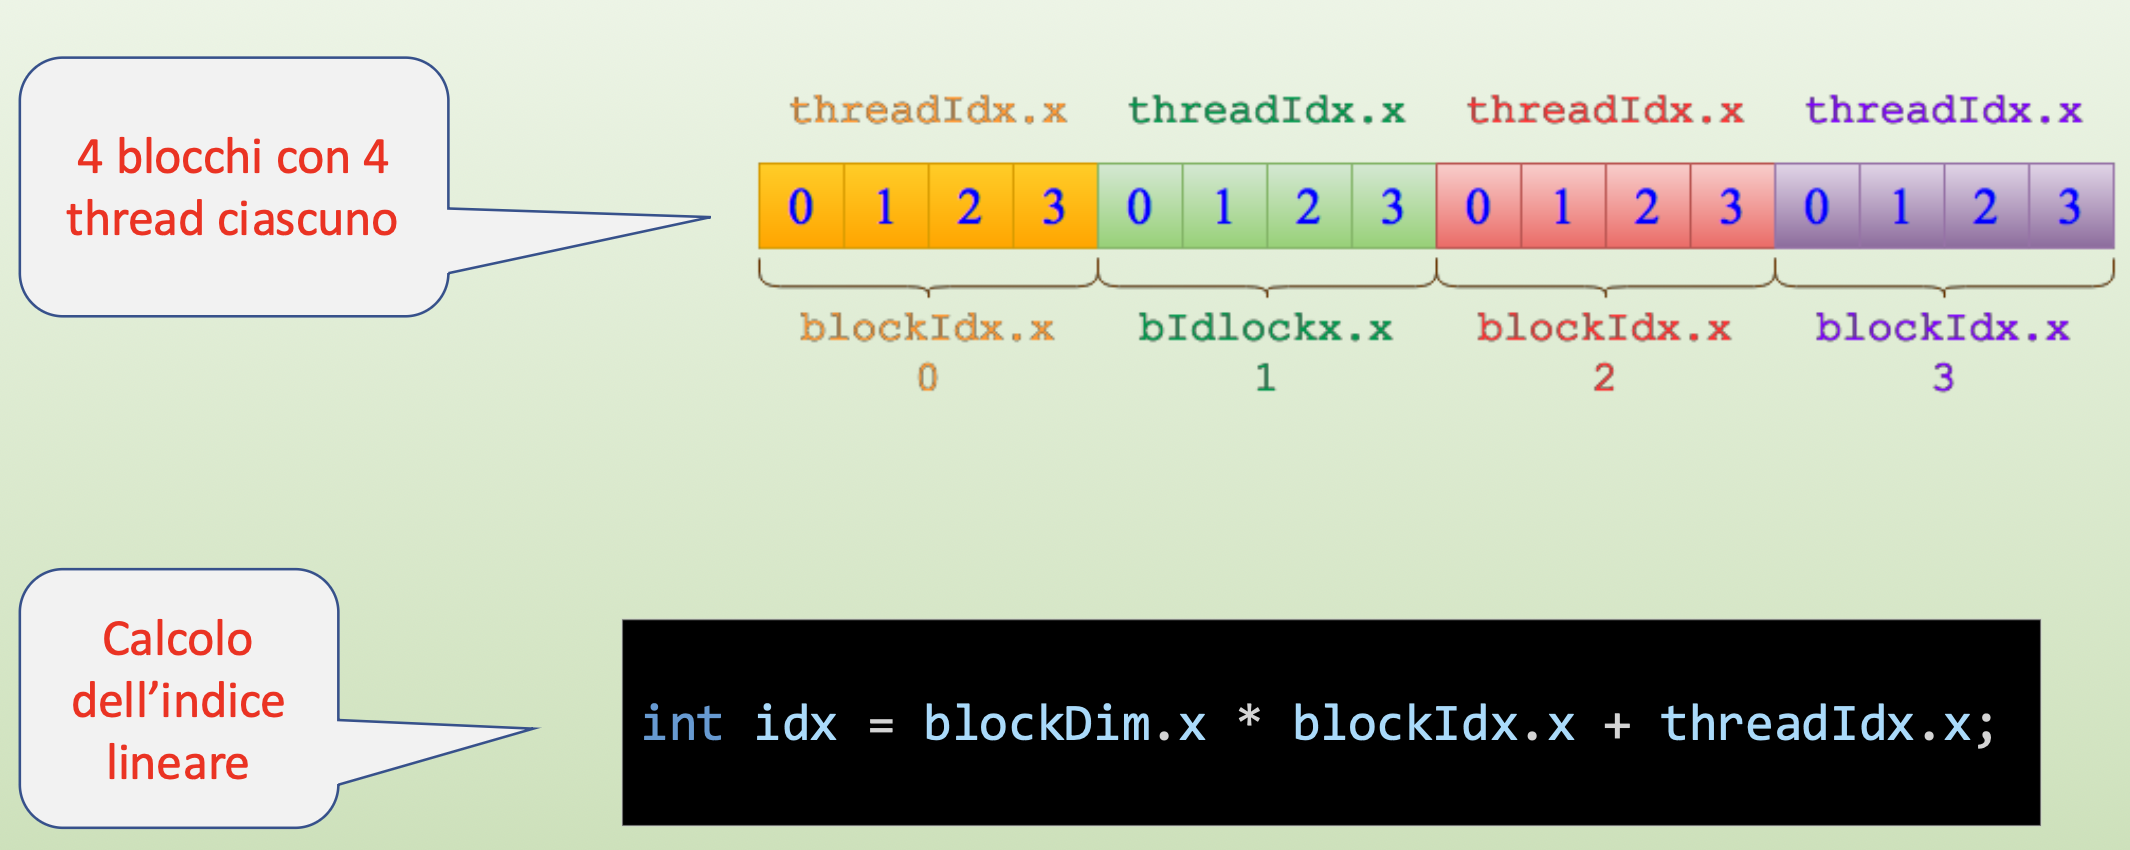
\includegraphics[width=0.8\textwidth]{images/grid1Dcoordinate1D.png}
    \caption{Organizzazione della griglia 1D e coordinate 1D}
\end{figure}

\subsection{Lancio di un kernel CUDA}
Quando prendo una funzione e la lancio con un kernel significa che prendo quella funzione e la lancio sulla GPU, i parametri di configurazione di esecuzione sono fatti in questo modo:
\begin{lstlisting}
    kernel<<<gridDim, blockDim>>>(args...);
\end{lstlisting}
Il primo valore \texttt{gridDim} specifica la dimensione della griglia di blocchi, mentre il secondo valore \texttt{blockDim} specifica la dimensione di ciascun blocco di thread. Gli argomenti \texttt{args...} rappresentano i parametri da passare al kernel.

\subsection{Kernel concorrenti}
Potrebbe verificarsi che numerosi kernel vengano lanciati sullo stesso host (dallo stesso processo o da processi diversi), potrei trovarmi nella situazione in cui ho diversi blocchi concorrenti sullo stesso device.

Esiste l'api \underline{cudaDeviceSynchronize} che permette di sincronizzare l'esecuzione dei kernel, significa che la cpu si sincronizza con tutti i kernel, praticamente il lancio del kernel diventa bloccante.

\subsection{Restrizioni del kernel}
\begin{itemize}
    \item Accede alla memoria globale
    \item Restituisce void
    \item non supporta numero variabile di argomenti, devono essere specificati
    \item non supporta le variabili statiche
    \item ha un comportamento asincrono rispetto al chiamante
\end{itemize}

\subsection{Memoria}
E' praticamente una trasposizione 1 a 1 della memoria in C, le funzioni servono per allocare memoria sul device in global memory (ricordasi che i thread accedono tutti alla global memory):
\begin{itemize}
    \item cudaMalloc: alloca memoria sul device
    \item cudaFree: dealloca memoria sul device
    \item cudaMemcpy: copia dati tra host e device
    \item cudaMemset: imposta un valore nella memoria del device
\end{itemize}
Il trasferimento e l'allocazione di memoria sono operazioni sincrone, l'host si ferma in attesa del completamento di queste operazioni.

cudaMalloc ritorna un doppio puntatore, che e' quello che viene passato ai kernel per puntare correttamente allo spazio di indirizzamento del device (memoria globale), la size e' in byte, il puntatore e' di tipo void\*:
\begin{lstlisting}
    cudaError_t cudaMalloc(void** devPtr, size_t size);
\end{lstlisting}

restituisce un codice di errore. La cudaFree e' quella che libera la memoria.

I puntatori su host e device sono diversi, non e' possibile fare assegnamenti tra uno e l'altro invece bisogna usare la cudaMemcpy.
